\documentclass[a4paper,12pt]{article} % Document class

% Packages
\usepackage[utf8]{inputenc} % Encoding
\usepackage{amsmath} % For mathematical formulas
\usepackage{graphicx} % For including images
\usepackage{hyperref} % For hyperlinks
\usepackage{titling} % For custom title
\usepackage{pdflscape} % For landscape pages
\usepackage{tabularx} % For flexible column widths
\usepackage[margin=2.5cm]{geometry} % Adjust the margin here (e.g., 2.5cm)
\usepackage{graphicx} % For including images
\usepackage{multirow}


% Set default path for images
\graphicspath{{../img/}}

% Prevent hyphenation globally
\hyphenpenalty=10000
\exhyphenpenalty=10000

\title{Web Technologies \\
        \large{Exercise Sheet 1 -- Web-Shop - Presentations and HTML}} % Title
\author{Team 3: Jiahui~Dai, Yana~Halamakh, Wei~Wei~Tang} % Author
\date{\today} % Date

\begin{document}

\maketitle % Create title
\hrule % Create a horizontal line
\tableofcontents % Create table of contents
\newpage



\section{General Questions}
\subsection{Task 1.1}


\subsection{Task 1.2}
\subsection{Communication Layers}

\begin{center}
    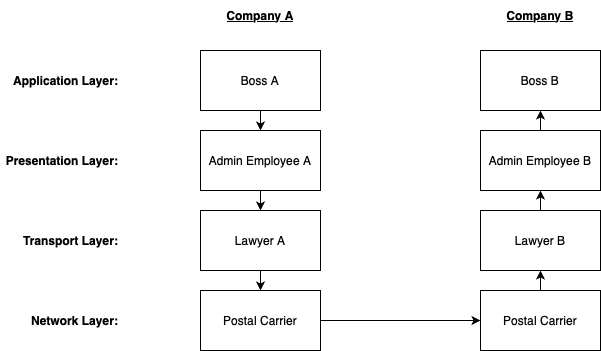
\includegraphics[width=.8\textwidth]{communication-layers.drawio.png}
\end{center}

% Application Layer: The bosses send messages through their administrative employees (Admin A and Admin B).
% Presentation Layer: Responsible for ensuring the message is encrypted before sending and decrypted upon receiving.
% Transport Layer: Handles the transmission of messages between Admin A and Admin B.
% Network Layer: Responsible for the routing and addressing of messages over the internet.

\section{Conceptual Model}
Please refer to  Figure~\ref{fig:task2} for the structural workflow model of our website.
% To redraw diagram.

\begin{figure}[h]
    \centering
    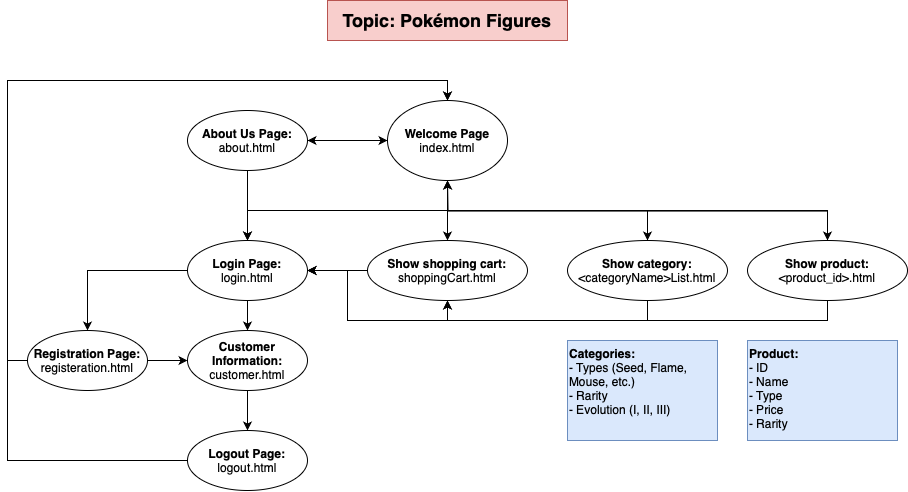
\includegraphics[width=\textwidth]{conceptual-model.drawio.png} % Adjust the path and file name
    \caption{Conceptual Model for Web-Shop}
    \label{fig:task2}
\end{figure}



% \section{\texttt{index.html}}
% Links: 
% \href{../src/index.html}{\texttt{index.html}}


% \section{\texttt{login.html}}
% Links: 
% \href{../src/login.html}{\texttt{login.html}}


% \section{\texttt{registration.html}}
% Links: 
% \href{../src/registration.html}{\texttt{registration.html}}


% \section{\texttt{logout.html}}
% Links: 
% \href{../src/logout.html}{\texttt{logout.html}}


% \section{\texttt{customer.html}}
% Links: 
% \href{../src/customer.html}{\texttt{customer.html}}


% \section{\texttt{about.html}}
% Links: 
% \href{../src/about.html}{\texttt{about.html}}


% \section{\texttt{<categoryName>List.html}}

% \begin{tabular}{|c|c|}
%     \hline
%     \textbf{Main Categories} & \textbf{Sub-Categories}\\
%     \hline
%     % Type
%     \multirow{3}{*}{Type} & Grass \\
%     \cline{2-2}
%     & Poison \\
%     \cline{2-2}
%     & Water \\
%     \hline
%     % Category
%     \multirow{4}{*}{Category} & Seed \\
%     \cline{2-2}
%     & Tiny Turtle \\
%     \cline{2-2}
%     & Turtle \\
%     \cline{2-2}
%     & Shellfish \\
%     \hline
% \end{tabular}


% \section{\texttt{<product\_id>.html}} 
% \begin{tabular}{|c|c|}
%     \hline
%     \textbf{ID} & \textbf{Name}\\
%     \hline
%     \#0001 & Bulbasaur\\
%     \hline
%     \#0002 & Ivysaur\\
%     \hline
%     \#0003 & Venusaur\\
%     \hline
%     \#0007 & Squirtle\\
%     \hline
%     \#0008 & Wartortle\\
%     \hline
%     \#0009 & Blastoise\\
%     \hline
% \end{tabular}






% END OF DOCUMENT
\begin{center}
    \vspace{5em}
    \textbf{END OF DOCUMENT}
\end{center}


\end{document}
